%; whizzy paragraph -pdf xpdf -latex ./whizzypdfptex.sh
%; whizzy-paragraph "^\\\\begin{frame}\\|\\\\emtext"
% latex beamer presentation.
% platex, latex-beamer でコンパイルすることを想定。 

%     Tokyo Debian Meeting resources
%     Copyright (C) 2012 Junichi Uekawa
%     Copyright (C) 2016 Nobuhiro Iwamatsu

%     This program is free software; you can redistribute it and/or modify
%     it under the terms of the GNU General Public License as published by
%     the Free Software Foundation; either version 2 of the License, or
%     (at your option) any later version.

%     This program is distributed in the hope that it will be useful,
%     but WITHOUT ANY WARRANTY; without even the implied warreanty of
%     MERCHANTABILITY or FITNESS FOR A PARTICULAR PURPOSE.  See the
%     GNU General Public License for more details.

%     You should have received a copy of the GNU General Public License
%     along with this program; if not, write to the Free Software
%     Foundation, Inc., 51 Franklin St, Fifth Floor, Boston, MA  02110-1301 USA

\documentclass[cjk,dvipdfmx,12pt]{beamer}
\usetheme{Tokyo}
\usepackage{monthlypresentation}

%  preview (shell-command (concat "evince " (replace-regexp-in-string "tex$" "pdf"(buffer-file-name)) "&")) 
%  presentation (shell-command (concat "xpdf -fullscreen " (replace-regexp-in-string "tex$" "pdf"(buffer-file-name)) "&"))
%  presentation (shell-command (concat "evince " (replace-regexp-in-string "tex$" "pdf"(buffer-file-name)) "&"))

%http://www.naney.org/diki/dk/hyperref.html
%日本語EUC系環境の時
\AtBeginDvi{\special{pdf:tounicode EUC-UCS2}}
%シフトJIS系環境の時
%\AtBeginDvi{\special{pdf:tounicode 90ms-RKSJ-UCS2}}

\newenvironment{commandlinesmall}%
{\VerbatimEnvironment
  \begin{Sbox}\begin{minipage}{1.0\hsize}\begin{fontsize}{8}{8} \begin{BVerbatim}}%
{\end{BVerbatim}\end{fontsize}\end{minipage}\end{Sbox}
  \setlength{\fboxsep}{8pt}
% start on a new paragraph

\vspace{6pt}% skip before
\fcolorbox{dancerdarkblue}{dancerlightblue}{\TheSbox}

\vspace{6pt}% skip after
}
%end of commandlinesmall

\title{東京エリアDebian勉強会\\Debian JP Project}
\subtitle{OSC2017 Tokyo/Spring 出張勉強会}
\author{岩松 信洋}
\date{2017年3月11日}
\logo{
\includegraphics[width=8cm]{image200607/openlogo-light.eps}}

\begin{document}

\begin{frame}
\titlepage{}
\end{frame}

\begin{frame}{Agenda}
  \begin{itemize}
   \item Debian とは?
   \item Debian Updates
   \item Debian 9 情報
   \item 今後のイベント
  \end{itemize}
\end{frame}

\section{Debian とは?}
\begin{frame}\begin{center}\Huge{Debian とは?}\end{center}\end{frame}

\begin{frame}{Debian とは?}

{\color{red}{フリー/オープン}}な{\color{red}{ユニバーサル}}オペレーティングシステム を作成しようとするボランティアベースのプロジェクト。

\begin{table}[htb]
  \begin{tabular}{|c|c|c|}
    \hline
    ディストリ & 企業 & ボランティア \\ \hline
    RHEL & RedHat & なし  \\ \hline
    CentOS & RedHat & あり \\ \hline
    Ubuntu  & Canonical & あり \\ \hline
    \color{red}{Debian}  & \color{red}{なし} & \color{red}{あり} \\ \hline
  \end{tabular}
\end{table}

\end{frame}

\begin{frame}{Debian とは?}
Linux カーネルだけではなく、FreeBSD や GNU/Hurd のカーネルを利用したOSも提供。

\begin{center}
%\includegraphics[width=0.3\hsize]{image201611/625px-NewTux.png}
%\includegraphics[width=0.3\hsize]{image201606/Freebsd-logo.jpg}\\
%\includegraphics[width=0.8\hsize]{image201606/hurd.png}
\end{center}

\end{frame}

\begin{frame}{Debian とは?}

  \begin{itemize}
  \item Debian 社会契約(オープンソースの定義の元)
  \item Debian フリーソフトウェアガイドライン
  \item Debian Policy
  \end{itemize}

\end{frame}

\begin{frame}{Debian とは?}

\begin{minipage}{0.45\hsize}
  \begin{itemize}
\item Ubuntu や Raspbian といったディストリビューションのベースとなっている \\
	Debian Derivatives (Debian 派生ディストリビューション調査と協力体制の整備)
  \end{itemize}
\end{minipage} 
\begin{minipage}{0.45\hsize}
 \begin{center} 
%   \includegraphics[width=1\hsize]{image201606/DebianFamilyTree1210.png}
% https://en.wikipedia.org/wiki/List_of_Linux_distributions#/media/File:DebianFamilyTree1210.svg
 \end{center}
\end{minipage}

\end{frame}

\begin{frame}{Debian とは?}
 世界規模で開発が行われており、63ヶ国、約1000名のDebian公式開発者が開発を行
 っている。パッケージメンテナや翻訳などの貢献者も入れるともっと多くの開発者が参加
 していることになる。
 \begin{center}
%  \includegraphics[width=0.7\hsize]{image201606/group_photo_t.jpg}
 \end{center}
\end{frame}

\begin{frame}{Debian とは?}
\begin{itemize}[<+->]
 \item 2016年11月の時点で、\pause 最新版は {\color{red}{Debian 8.6}} (コードネーム Jessie)、\pause
 パッケージ数は{\color{red}{約43000}}を提供、\pause
 公式にサポートするCPUアーキテクチャは{\color{red}{10}}。\pause
 \item {\color{red}{約2年毎}}にリリース
% \begin{center}
% \includegraphics[width=0.7\hsize]{image201605/i4282a1da3049189bccafa8929c4df0ab.png}
% \end{center}
 \item 次のリリース (コードネーム: {\color{red}{}}Stretch)は 2017年Q2またはQ3の予定
 \item コードネームはトイ・ストーリのキャラクターを採用している。
  \begin{center}
%  \includegraphics[width=0.5\hsize]{image201606/toy.jpg}
  \end{center}
\end{itemize}
\end{frame}

\begin{frame}{Debian とは?}
  \begin{center}
%  \includegraphics[width=0.5\hsize]{image201611/chin_.jpg}
% buz の顎拡大画像
  \end{center}
\end{frame}

\if 0
\begin{frame}{Debian とは?}
どこで使われているのか?\pause
Linux ディストリビューションのベース

  \begin{center}
%   \includegraphics[width=0.5\hsize]{image201606/ubuntu.png}
  \end{center}

\end{frame}

\begin{frame}{Debian とは?}
Webサーバとして利用されてる(2016/06時点)

  \begin{center}
%  \includegraphics[width=0.5\hsize]{image201606/w3techs.png}
  \end{center}
  \tiny{\url{http://w3techs.com/technologies/details/os-linux/all/all}}

\end{frame}

\begin{frame}{Debian とは?}
組込デバイスのベースOSとして利用されている

 \begin{center}
% \includegraphics[width=0.5\hsize]{image201606/bbb-logo.jpeg}
%%  http://www.tech-villa.com/images/kallyas_images/blog_images/beagleboneblack_logo.jpg
 \end{center}
 \url{http://beagleboard.org/}

 \begin{center}
% \includegraphics[width=0.2\hsize]{image201606/rpi-logo.png}
%  https://www.raspberrypi.org/wp-content/uploads/2015/08/raspberry-pi-logo.png
 \end{center}
 \url{https://www.raspberrypi.org/}

 \end{frame}

\begin{frame}{Debian とは?}

\begin{itemize}
\item ISS (国際宇宙ステーション)
\begin{center}
% \includegraphics[width=0.5\hsize]{image201606/STS-134_International_Space_Station_after_undocking}
 https://ja.wikipedia.org/wiki/%E5%9B%BD%E9%9A%9B%E5%AE%87%E5%AE%99%E3%82%B9%E3%83%86%E3%83%BC%E3%82%B7%E3%83%A7%E3%83%B3#/media/File:STS-134_International_Space_Station_after_undocking.jpg
\end{center}
{\tiny \url{https://training.linuxfoundation.org/why-our-linux-training/training-reviews/linux-foundation-training-prepares-the-international-space-station-for-linux-migration}}

\item Steam (ゲームPC OS)
\item NAS、ルータ
\item etc..
\end{itemize}

\end{frame}

\fi

\begin{frame}{Debian とは?}
まとめると\pause
\begin{itemize}[<+->]
\item Debianはフリー/オープンなオペレーティングシステム (OS)を作成しようとするボランティアベースのプロジェクト。
\item 自分たちの考えるフリーという言葉に関する定義、開発目的、パッケージングポリシーを厳格に決めている。
\item 世界中に1000人以上の開発者がおり、他のディストリビューションのベースとして採用されている。
\item 約2年毎にリリースが行われ、多くのパッケージとアーキテクチャをサポートしている。次期リリースは2017年Q2からQ3。
\item 上記のような特徴から様々なところで利用されているLinuxディストリビューションである。
\end{itemize}

\end{frame}

\begin{frame}{Debian JP Project とは?}
\pause
\begin{itemize}[<+->]
\item 日本でDebianを普及させることを目的とした任意団体。
\item Debian の日本語による情報発信、ユーザとの情報交換、Debian 開発者、パッケージメンテナの育成など。
\end{itemize}
\end{frame}


\begin{frame}
\frametitle{Debian勉強会}
\begin{itemize}
 \item 2005年1月開始
 \item Debian Developer 上川さん発起人
\item 東京と関西で月に一回コンスタントに開催しているDebian開発者、ユーザによる勉強会。
\end{itemize}
\end{frame}

\begin{frame}

\frametitle{Debian勉強会:解決したい内容}
\begin{itemize}
 \item<1-> 問題
       \begin{itemize}
	\item MLとIRCで情報交換していた
	\item face-to-faceであう場所がない
	\item まとまったドキュメントが出てこない
       \end{itemize}
 \item<2-> Debian勉強会の提案
       \begin{itemize}
	\item 定期的に集まる
	\item 資料を必ず作成する。(GPLで!) \\
	  {\small \url{git://anonscm.debian.org/tokyodebian/monthly-report.git}}
       \end{itemize}
\end{itemize}

\end{frame}

\begin{frame}
 \frametitle{Debian勉強会:実際}
 \begin{itemize}
  \item Debian Weekly News Quiz
  \item Debian 界隈やパッケージング関連の話題など専門の人に話を聞く
  \item 前回の内容(東京):\\
	\begin{itemize}
	\item 場所: 朝日ネットさん
	\item Debian 9 Stretch に向けた Debian Bug Squashing Party
        \item 9名が参加。17個のバグレポート対応。
	\end{itemize}
  \item 各地のイベントでDebian普及活動。 
	\begin{itemize}
	  \item OSC京都、KOF、OSC群馬、OSC沖縄、OSC北海道など
	  \item Debian/Ubuntu ユーザミートアップ in 札幌を開催
	\end{itemize}
 \end{itemize}
\end{frame}

\begin{frame}
 \frametitle{Debian Mini Conference 2016}
 \begin{itemize}
      \item 2016年12月10日 サイボウズ株式会社さん(東京・日本橋)で開催
      \item Webサイト: \url{http://miniconf.debian.or.jp/}
      \item 13個の発表。76名の参加者。
 \end{itemize}
\end{frame}

\begin{frame}\begin{center}\Huge{Debian Updates}\end{center}\end{frame}

\begin{frame}{Debian Updates}
\begin{itemize}[<+->]
\item 2017/01/14: Updated Debian 8: 8.7
 \begin{center}
 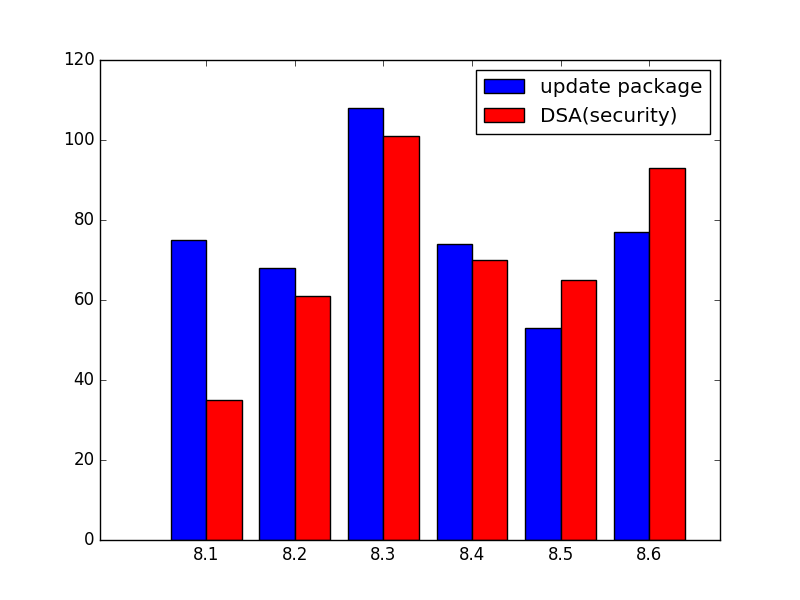
\includegraphics[width=0.6\hsize]{image201611/stable-updates.png}
 \end{center}
\end{itemize}

\end{frame}

\section{Debian Updates}

\begin{frame}{Thunderbird が Debian / unstable に}

\begin{itemize}
\item 商標問題で Firefox が Iceweasel として、Thunderbird が Icedove として
提供されてきたが、Iceweasel から1年遅れでIcedoveも Thunderbirdにとして
提供されるようになった。
\item 残念なことに Debian 9には入らないが、backports などを使って使用
できるようになる可能性がある。
\end{itemize}

\begin{center}

\includegraphics[width=0.6\hsize]{image201703/img_5609_thunderbirdeditadoopenlogodebian1.jpg}
\end{center}

Source: \url{https://lists.debian.org/debian-devel-announce/2017/02/msg00004.html}
IMG: \url{http://cdn.sejalivre.org/uploads/2012/03/img_5609_thunderbirdeditadoopenlogodebian1.jpg}

\end{frame}

\begin{frame}{SHA1 と RIPE-MD/160 によってサインされたパッケージアップロードを拒否}

Source: \url{https://lists.debian.org/debian-devel-announce/2017/02/msg00007.html}

Archive no longer accepts uploads signed using SHA-1 or RIPE-MD/160

\end{frame}

\begin{frame}{Debian Installer RC1, RC2 リリース}
installer RC , RC2

ブースで配っています。
\end{frame}


\begin{frame}{Debian リポジトリアーカイブの圧縮方法とチェックサムの変更}

\begin{itemize}
\item 今まで リポジトリアーカイブは .gz と bz2 で提供されてきたが、gz と xz に。
\item 上記アーカイブのハッシュ値提供から、SHA1が無効化。MD5とSHA256のみに切り替
え。
\end{itemize}
%前はMD5も無効化される予定だった。

%https://lists.debian.org/debian-devel-announce/2016/03/msg00006.html
Source: \url{https://lists.debian.org/debian-devel-announce/2016/11/msg00005.html}

\end{frame}




\section{次期リリース Debian 9 について}
\begin{frame}\begin{center}\Huge{次期リリース Debian 9 について}\end{center}\end{frame}

\begin{frame}{次期リリース Debian 9 について}% [containsverbatim]
Debian 9 のコードネームは \pause \\
 \begin{center}
{\Huge stretch} \pause
% \includegraphics[width=0.8\hsize]{image201606/stretch.jpg}
 \end{center}
\end{frame}

\begin{frame}{次期リリース Debian 9 について}% [containsverbatim]

スケジュール

\begin{itemize}
\item 2016年11月5日: transitions freeze
\item 2017年1月5日: "Soft" freeze
\item \color{red}{2017年2月5日: Full freeze} $\leftarrow$ いまここ
\end{itemize}

RCバグ、パッケージプライオリティがoptional か extra の important バグ、翻訳
ドキュメント関連のバグが修正可能な状態。現在のバグは\color{red}{153}個。

%\url{https://udd.debian.org/bugs.cgi?release=wheezy_and_sid&patch=ign&merged=ign&done=ign&fnewerval=7&rc=1&sortby=id&sorto=asc&ctags=1&ctags=1&cdeferred=1#results

\end{frame}

\begin{frame}{次期リリース Debian 9 について}% [containsverbatim]

サポートアーキテクチャ
\begin{itemize}
\item i386アーキテクチャのサポートCPUをi686以降に変更
\item サポートされるアーキテクチャ \\
  amd64, i386, armel, armhf, arm64, mips, mipsel, {\color{red}{mips64el}}, ppc64el, s390x
\item サポートから外れるアーキテクチャ \\
  powerpc 
\end{itemize}

\tiny{\url{https://lists.debian.org/debian-devel-announce/2016/10/msg00008.html}}

\end{frame}

\begin{frame}{次期リリース Debian 9 について}% [containsverbatim]

サポートアーキテクチャ
 \begin{center}

UPDATE IMAGE
 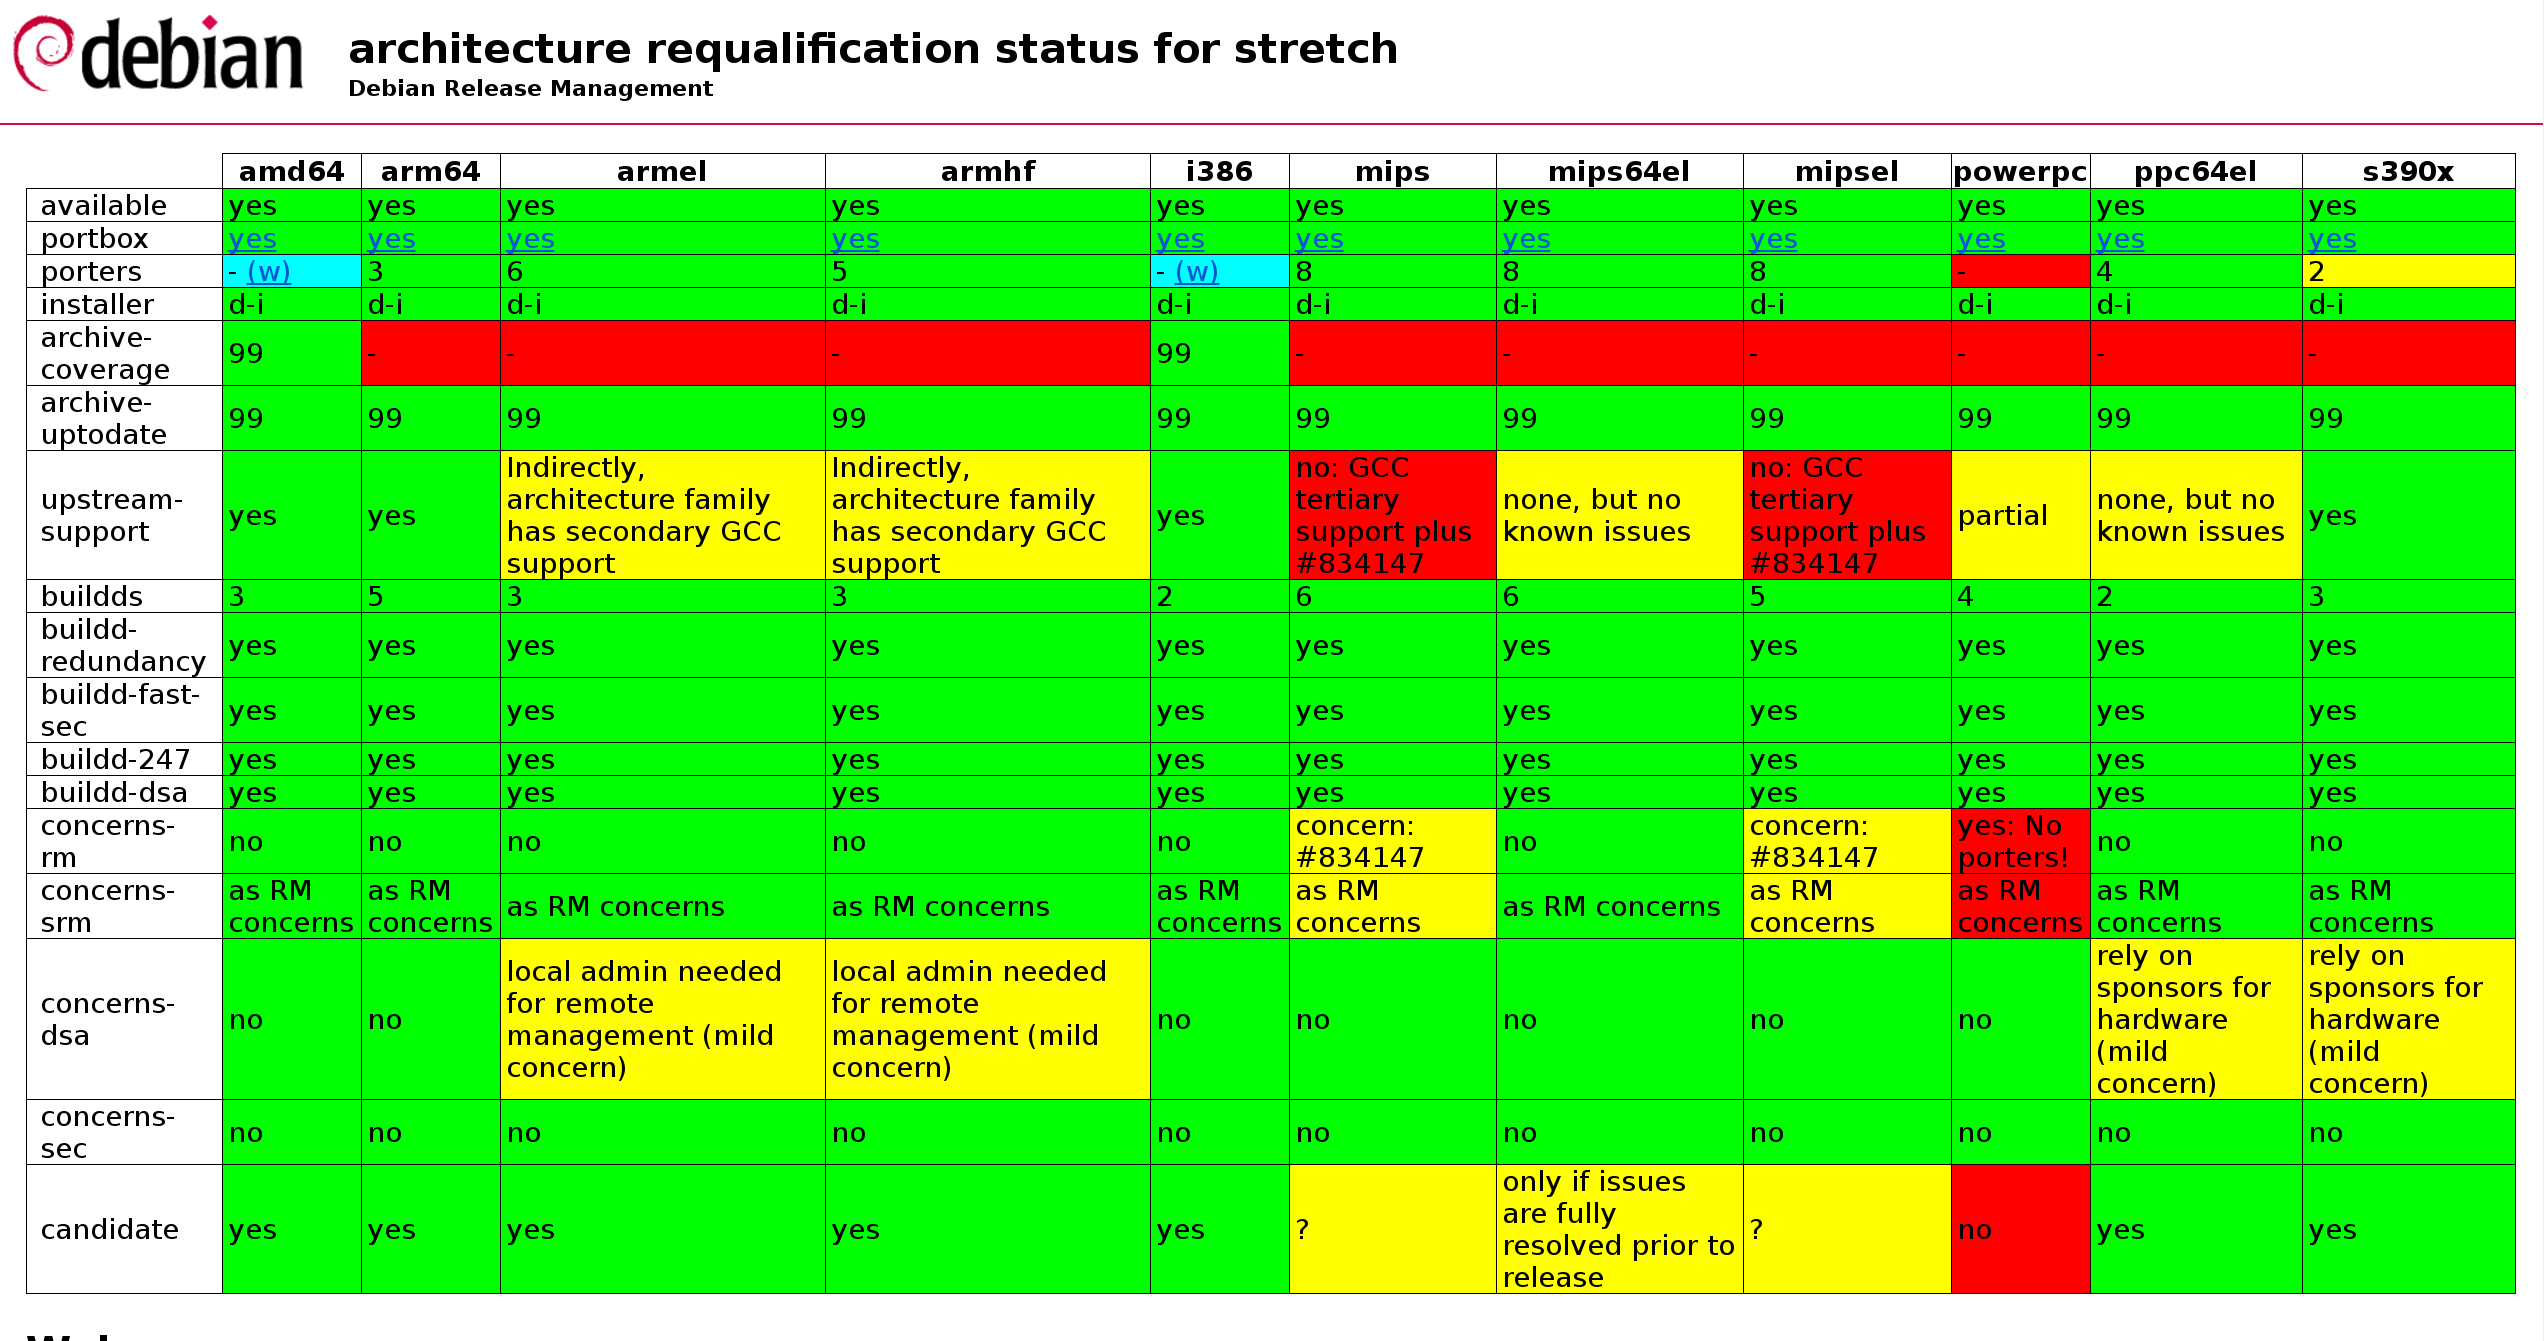
\includegraphics[width=1.0\hsize]{image201611/stretch-arch-requalification.png}
 \end{center}

\end{frame}

\begin{frame}{次期リリース Debian 9 について}% [containsverbatim]

テーマ\\
Juliette Taka Belin さんが作成した Soft waves に決定。
 \begin{center}
% \includegraphics[width=0.8\hsize]{image201611/attachment_wallpaper.png}
 \end{center}

\end{frame}


\begin{frame}{次期リリース Debian 9 について}% [containsverbatim]

ソフトウェア
\begin{itemize}
\item Linux カーネルは 4.9.x
\item ツールチェイン(GCC 6, binutils 2.27, glibc 2.24), LLVM 3.8, 3.9
\item Perl 5.24.1 ,Python 2.7.13/3.5.1, Ruby 2.3.3 ,PHP 7.1.1, Go 1.7.4, OpenJDK 8
\item GNOME 3.22, KDE 5.8.4, Xfce 4.12.1, lxde 0.99.2, lxqt 0.11.1
\item MySQL 5.7.17, MariaDB 10.0.28, PostgreSQL 9.6.2, sqlite 3.16.2
\item OpenSSL 1.1.0e
\item クロスコンパイラがデフォルトでサポート
\item デバッグシンボルパッケージがデフォルトで提供
\end{itemize}

\end{frame}

\section{日本語によるDebianの情報}
\begin{frame}\begin{center}\Huge{日本語によるDebianの情報}\end{center}\end{frame}

\begin{frame}{日本語によるDebianの情報}
\begin{itemize}
  \item Debian JP Project \\
      \url{http://www.debian.or.jp}
  \item 東京エリアDebian勉強会\\
      \url{http://tokyodebian.alioth.debian.org}
  \item 関西エリアDebian勉強会 \\
      \url{https://wiki.debian.org/KansaiDebianMeeting}
  \item Twitter \\
      \url{@debian_jp}
  \item G+ コミュニティ \\
      \url{https://plus.google.com/u/0/communities/106942835439686570073}
 
\end{itemize}
\end{frame}

\section{今後のイベント}
\begin{frame}\begin{center}\Huge{今後のイベント}\end{center}\end{frame}

\begin{frame}{今後のイベント}
\begin{itemize}

\item 3月19日 第121回関西Debian勉強会(10 周年記念会)
  \begin{itemize}
      \item 江之子島文化芸術創造センター/enoco, Room 12 
      \item \url{https://k-of.jp/2016/}
  \end{itemize}
\item 4/15 第14x回東京エリアDebian勉強会
  \begin{itemize}
      \item 株式会社 朝日ネット(東京/銀座)
      \item \url{http://tokyodebian.alioth.debian.org/2016-11.html}
  \end{itemize}
\item  Debian 9 リリースパーティ (日程未定)
  \begin{itemize}
      \item 場所は未定
  \end{itemize}
\end{itemize}
\end{frame}

\begin{frame}{Debconf17}
  \begin{itemize}
      \item カナダ・モントリオール
      \item Webサイト: \url{https://debconf17.debconf.org/}
      \item 8月6日から12日まで
      \item 4月まで発表者受付中
  \end{itemize}

\begin{center}

\includegraphics[width=0.8\hsize]{image201703/debconf17-logo.eps}
\end{center}

オリンピックセンターをモチーフにしたロゴ。

\end{frame}

\begin{frame}{質問}
\begin{center}
何か質問はありますか?
\end{center}
\end{frame}

\end{document}

;;; Local Variables: ***
;;; outline-regexp: "\\([ 	]*\\\\\\(documentstyle\\|documentclass\\|emtext\\|section\\|begin{frame}\\)\\*?[ 	]*[[{]\\|[]+\\)" ***
;;; End: ***
